\section{Evaluation and Empirical Results}
\label{sec:evaluation}

We evaluate \texttt{peptide\_extractor} using two complementary frameworks: (1) reference-free completeness and citation-grounding verification for unlabeled corpus-scale runs, and (2) normalized precision/recall/F1 benchmarking against manually curated golden entries.

\subsection{Reference-Free Grounding and Completeness}
For any extracted \texttt{PeptideEntry} and its source full text, \texttt{evaluate\_extraction()} (\texttt{evaluation.py}) computes:
\begin{itemize}
    \item \textbf{Completeness Rate:} Fraction of non-null fields out of 16 standard fields (or 17 when \texttt{peptide\_conjugate\_mixture} is \texttt{conjugate} or \texttt{mixture}, requiring \texttt{conjugate\_partner}).
    \item \textbf{Groundness Rate:} Fraction of checkable non-null fields verified against the source document:
    \begin{enumerate}
        \item \emph{Citation-Grounded Fields:} The 12 \texttt{EvidenceSpan} fields are resolved to their cited \texttt{Node} text via \texttt{get\_node\_by\_id()} and verified by an LLM judge (\texttt{deepseek-r1:8b} via Ollama).
        \item \emph{Verbatim Protocol:} \texttt{preparation\_protocol} is checked via exact substring match or \texttt{rapidfuzz} partial ratio $\ge 90.0$.
        \item \emph{Detection Methods:} Individual comma-separated techniques are matched against the full text (grounded if $\ge 80\%$ of listed methods match with partial ratio $\ge 90.0$).
    \end{enumerate}
\end{itemize}

\Cref{fig:eval_boxplots} and \Cref{fig:corpus_stats} show corpus-level evaluation distributions, column completion rates, peptide length distributions, and per-paper extraction counts generated by the visualization framework.

\begin{figure}[htbp]
\centering
\begin{subfigure}[b]{0.48\textwidth}
    \centering
    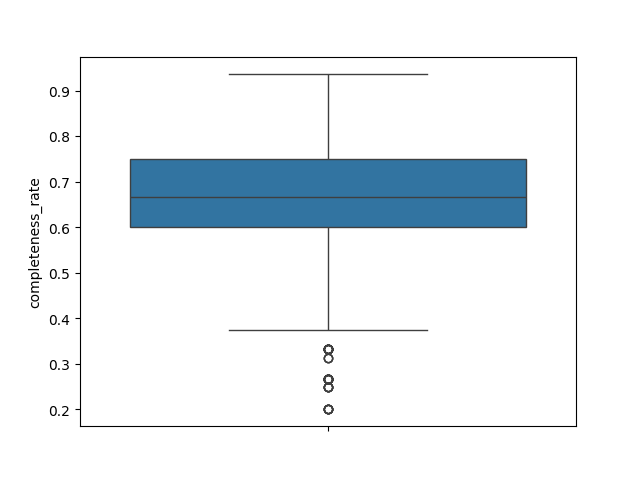
\includegraphics[width=\textwidth]{completeness_boxplot.png}
    \caption{Field completeness rate distribution}
    \label{fig:comp_box}
\end{subfigure}
\hfill
\begin{subfigure}[b]{0.48\textwidth}
    \centering
    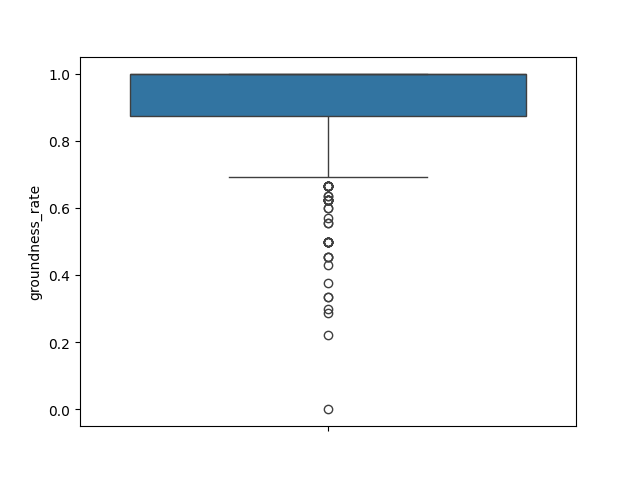
\includegraphics[width=\textwidth]{groundness_boxplot.png}
    \caption{Citation groundness rate distribution}
    \label{fig:ground_box}
\end{subfigure}
\caption{Reference-free evaluation distributions across extracted \texttt{PeptideEntry} records.}
\label{fig:eval_boxplots}
\end{figure}

\begin{figure}[htbp]
\centering
\begin{subfigure}[b]{0.48\textwidth}
    \centering
    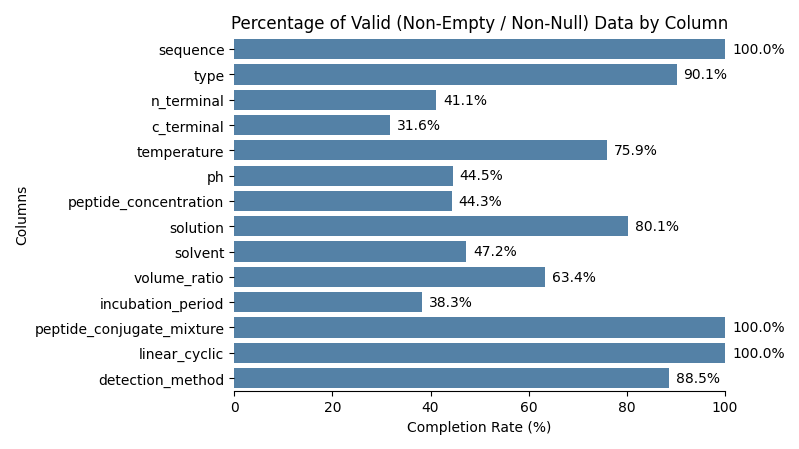
\includegraphics[width=\textwidth]{column_completion_final.png}
    \caption{Per-column completion rates}
    \label{fig:col_comp}
\end{subfigure}
\hfill
\begin{subfigure}[b]{0.48\textwidth}
    \centering
    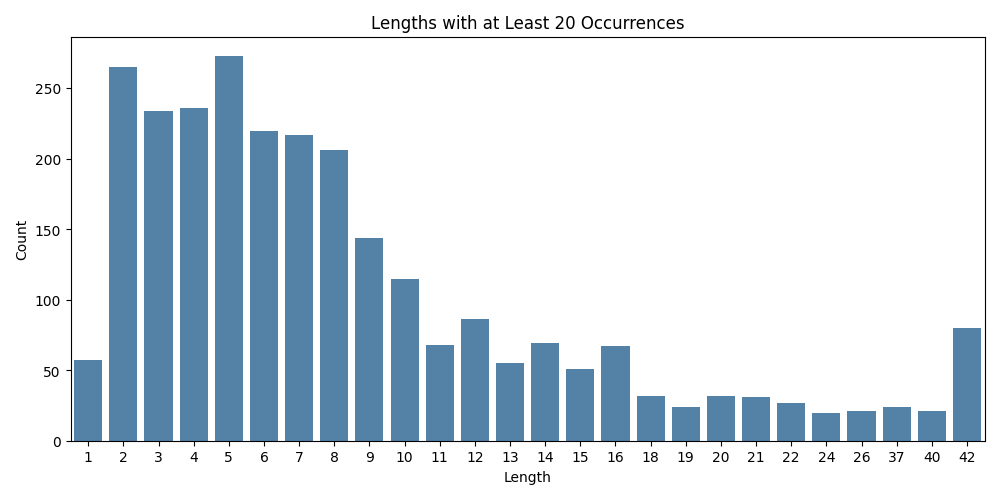
\includegraphics[width=\textwidth]{lengths_updated.png}
    \caption{Extracted peptide length distribution}
    \label{fig:len_dist}
\end{subfigure}
\caption{Extracted dataset characteristics across processed publications.}
\label{fig:corpus_stats}
\end{figure}

\subsection{Golden Dataset Benchmarking}
\texttt{benchmark\_run\_against\_golden()} (\texttt{golden\_benchmark.py}) compares LLM runs against \texttt{ExtractionMode.MANUAL} (\texttt{run\_identifier=0}) after canonicalizing terminal caps (\texttt{Ac} $\rightarrow$ \texttt{acetylation}, \texttt{NH2} $\rightarrow$ \texttt{amidation}), solvent tokens (\texttt{HFIP}/\texttt{HFP} $\rightarrow$ \texttt{hfp}), volume ratios, and numeric tolerances ($\pm 1.5\,^\circ\text{C}$ temperature, $\pm 0.2$ pH, $\pm 10\%$ relative concentration and incubation period). Entries are grouped by $(\text{pmid}, \text{sequence})$ and matched via greedy bipartite matching.

\Cref{tab:dev_benchmark} summarizes iterative progression across six runs on the 10-paper development slice (\texttt{DEV\_BENCHMARK\_PMIDS}: 56 manual sequences, 530 condition rows: 253 assembling, 277 non-assembling).

\begin{table}[htbp]
\centering
\caption{Development benchmark results across 10 multi-table golden papers (56 sequences, 530 condition rows).}
\label{tab:dev_benchmark}
\small
\begin{tabular}{@{}llcccccc@{}}
\toprule
\textbf{Run} & \textbf{Configuration} & \textbf{Seq R} & \textbf{Seq P} & \textbf{Seq F1} & \textbf{Rows} & \textbf{Matched} & \textbf{Cond P} \\
\midrule
Run 1 & Baseline (text, V4) & 28.6\% & 69.6\% & 40.5\% & 24 & 17 & 70.8\% \\
Run 2 & Multi-entry prompt (V5) & 28.6\% & 59.3\% & 38.6\% & 30 & 19 & 63.3\% \\
Run 3 & Mode A: Direct raw PDF & 91.1\% & 89.5\% & 90.3\% & \textbf{527} & \textbf{371} & 70.4\% \\
Run 4 & Mode C: PDF $\rightarrow$ text (V6) & 33.9\% & 82.6\% & 48.1\% & 90 & 67 & \textbf{74.4\%} \\
Run 5 & Mode B2: Table images (1-pass) & \textbf{92.9\%} & \textbf{91.2\%} & \textbf{92.0\%} & 359 & 258 & 71.9\% \\
Run 6 & Mode B1: Table images (2-pass) & 89.3\% & 83.3\% & 86.2\% & 444 & 302 & 68.0\% \\
\bottomrule
\end{tabular}
\end{table}

\subsection{Key Empirical Findings}
\begin{enumerate}
    \item \textbf{Visual Table Access is Critical:} Text-only GROBID conversion (Run~4) recovered only $33.9\%$ of sequences and $67/530$ condition rows ($12.6\%$). Passing cropped table images (Run~5) boosted sequence F1 to $92.0\%$ ($52/56$ sequences), while direct raw PDF (Run~3) achieved $90.3\%$ sequence F1 and matched $371/530$ condition rows ($70.0\%$: $57.3\%$ assembling recall, $81.6\%$ non-assembling recall).
    \item \textbf{Two-Pass Factoring Recovers Paper-Wide Defaults:} Single-pass table-image extraction (Run~5) achieved high sequence F1 ($92.0\%$) but frequently omitted paper-wide defaults under high row-count output---recovering temperature on only $40/258$ rows and incubation period on $23/254$ rows. Adding Pass~1 shared-condition extraction and deterministic merging (Run~6) increased matched rows from $258$ to $302$ ($+17\%$), restoring temperature coverage to $301/302$ ($99.7\%$ normalized accuracy) and incubation period coverage to $268/298$ ($92.2\%$ accuracy).
    \item \textbf{Remaining Field Normalization Gaps:} Across visual runs (Runs~3, 5, 6), normalized accuracy on \texttt{c\_terminal} ($4.0\%$--$24.3\%$) and \texttt{detection\_method} ($6.6\%$--$11.0\%$) lags behind \texttt{type} ($77.7\%$--$94.2\%$), \texttt{n\_terminal} ($91.4\%$--$96.8\%$), and \texttt{linear\_cyclic} ($93.0\%$--$97.7\%$), primarily due to differing conventions for amidated/free C-termini and per-method vs.\ per-experiment entry splitting in the golden dataset.
\end{enumerate}
